  %%%%%%%%%%%%%%%%%%%%%%%%%%%%%%%%%%%%%%%%%%%%%%%%%%%%%%%%%%%%%%%%%%%%%%
% LaTeX Example: Project Report

%%% Preamble
\documentclass[paper=a4, fontsize=11pt, abstract=on]{scrartcl}
\usepackage[T1]{fontenc}
\usepackage{fourier}
\usepackage{tabularx}
\usepackage[utf8]{inputenc}
\usepackage{hyperref}





\usepackage{listings}
\usepackage{color}

\definecolor{dkgreen}{rgb}{0,0.6,0}
\definecolor{gray}{rgb}{0.5,0.5,0.5}
\definecolor{mauve}{rgb}{0.58,0,0.82}
\lstset{frame=tb,
  language=[Visual]C++,
  aboveskip=3mm,
  belowskip=3mm,
  showstringspaces=false,
  columns=flexible,
  basicstyle={\small\ttfamily},
  numbers=none,
  numberstyle=\tiny\color{gray},
  keywordstyle=\color{blue},
  commentstyle=\color{dkgreen},
  stringstyle=\color{mauve},
  breaklines=true,
  breakatwhitespace=true,
  tabsize=3
}
\usepackage{graphicx}
\usepackage{caption}
\usepackage{subcaption}

\usepackage[english]{babel}															% English language/hyphenation
\usepackage[protrusion=true,expansion=true]{microtype}	
\usepackage{amsmath,amsfonts,amsthm} % Math packages

\usepackage{url}
%\usepackage[hang, small,labelfont=bf,up,textfont=it,up]{caption}


%%% Custom sectioning
\usepackage{sectsty}
\allsectionsfont{\normalfont\scshape}
\usepackage{float}
\usepackage{amsmath}
\usepackage{mathtools}
\usepackage{ragged2e}

\usepackage{nomencl}
\makenomenclature

%%% Custom headers/footers (fancyhdr package)
\usepackage{fancyhdr}
\pagestyle{fancyplain}
\fancyhead{}											% No page header
\fancyfoot[L]{}											% Empty 
\fancyfoot[C]{}											% Empty
\fancyfoot[R]{\thepage}									% Pagenumbering
\renewcommand{\headrulewidth}{0pt}			% Remove header underlines
\renewcommand{\footrulewidth}{0pt}				% Remove footer underlines
\setlength{\headheight}{13.6pt}
   \renewcommand*\abstractname{Summary}

%%% Equation and float numbering
\numberwithin{equation}{section}		% Equationnumbering: section.eq#
\numberwithin{figure}{section}			% Figurenumbering: section.fig#
\numberwithin{table}{section}				% Tablenumbering: section.tab#


%%% Maketitle metadata

\newcommand{\horrule}[1]{\rule{\linewidth}{#1}} 	% Horizontal rule

\title{
		%\vspace{-1in} 	
		\usefont{OT1}{bch}{b}{n}
		\normalfont \normalsize \textsc{} \\ [25pt]
		
\includegraphics[width=0.3\linewidth]{ubc.png} \\
		%
\includegraphics[width=0.4\linewidth]{tru}		
		\horrule{0.5pt} \\[0.2cm]
		\huge 502 Mini-Project \#2 : Flow due to Oscillating Plate  \\
		\horrule{2pt} \\[0.005cm]
}
\author{
		\normalfont 								\normalsize
        Jerin Roberts\\[-5pt]		\normalsize
        \today
}
\date{}




%%% Begin document
\begin{document}
\maketitle
\begin{center}
\begin{tabular}{l r}


Supervisor: & Dr. Dana Grecov  \\ % supervisor
Locations: & University of British Columbia


\end{tabular}
\end{center}



\newpage
\tableofcontents
\listoffigures
\listoftables
\newpage
\lstset{language=[Visual]C++}
\section{Overview}



 The problem of an oscillating plate bounding a fluid has lots of applications in a broad range of engineering and medical fields. The are several examples of problems inclduing oscillating plates which will be discussed in this report.
\section{Flow Due to an oscillating plate}
\subsection{Problem Overview}
First lets consider an infinite flat plate containing an infinite dept of fluid relative to the affect range. The plate executes sinusoidal oscillations parallel to the itself as shown in the diagram \ref{osc}.

\begin{figure}[H]
\centering
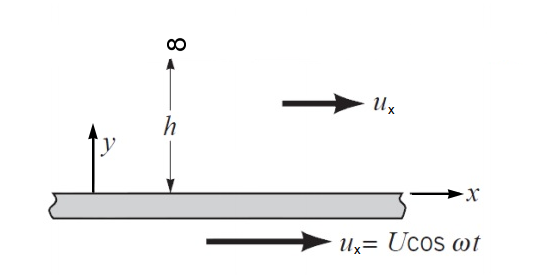
\includegraphics[width=0.85\linewidth]{di}
\caption{Calculated Order of Accuracy}
\label{ord}
\end{figure}



 The problem is to find a solution to the flow after all transients have died out. This simplifies the problem as there are no initial conditions to satisfy. This problem is often referred to as stokes second problem. We begin solving by finding the simplified governing equations from the generalized non-dimensional differential navier stokes equations \ref{nav}. This can written as a 1D problem as we are only concerned with the velocity profile $u_x$ in the y direction, ie $u-z$ and $u_y$ are considered to be small and equal to zero. These assumptions lead to many cancellations and result in the governing equations for the problem \ref{gov}



 \begin{equation}
\label{gov}
\frac{\partial u_x}{\partial t} = \eta \frac{\partial^2 u_x}{\partial y^2}
\end{equation} 




 \begin{equation}
\label{b1}
u(0,t) = U\cos \omega t
\end{equation}

 
  \begin{equation}
\label{b2}
u(0,\infty) = bounded = 0
\end{equation}

\subsection{Separation}
Since the period of the oscillations of the plate introduces a time scale, no similarity solution exists to this problem. By considering the equations governing the fluid it may be expected that $u_x$ will also oscillate with the same frequency relative to the movement of the plate, with however a phase shift due to the shear slip between fluid layers. In the steady state therefore the flow variables must have a periodicity equivalent to the periodicity of the motion of the plate. Therefore we will consider a separable solution of the form shown in equation \ref{51}.

 \begin{equation}
\label{51}
u = e^{i\omega t}f(y)
\end{equation}


where the solution will be considered the real part of the right-hand side. Because $f(y)$ is complex, the velocity of the fluid $u(y,t)$ is able to have a phase difference relative to the wall velocity $U\cos \omega t$. Substitution of Eq. \ref{51} into the governing equation \ref{gov} gives

\begin{equation}
\label{52}
i\omega f(y) = \eta \frac{d^2f(y)}{dy^2}
\end{equation}

This is an equation with constant coefficients and must have exponential solutions. Substitution of a solution of the form $f = exp(ky)$ gives $k = \sqrt{i\omega / \eta} \pm(i+1) \sqrt{\omega /2 \eta}$ where the two square roots of i have been used. Consequently, the solution of Eq. \ref{53} is


\begin{equation}
\label{53}
f(y) = Ae^{-(1+i)y\sqrt{\omega/2\eta}}+Be^{(1+i)y\sqrt{\omega/2\eta}}
\end{equation}


The condition (9.50), which requires that the solution must remain bounded at $y = \infty$, needs B = 0. The solution \ref{51} then becomes

\begin{equation}
\label{54}
u(y,t) = Ae^{i\omega t}e^{-(1+i)y\sqrt{\omega/2\eta}}
\end{equation}


After applying the surface boundary condition \ref{51} we find A to be equal to U. After considering on the real part of Eq.\ref{w4}, we finally obtain the velocity distribution over the oscillating plate:

\begin{equation}
\label{55}
u(y,t) = Ue^{-\omega t}\cos\Big(\omega t - y\sqrt{\omega/2\eta}\Big)
\end{equation}

The cosine term in Eq. \ref{55} ris a representation of a wave signal propagating in the direction of y , while the exponential term represents the amplitude decay in that propagating wave. The flow therefore resembles a damped wave as displayed in figure \ref{result}. On an interesting note the problem to be clear is purely a diffusion problem and not wave-propagation problem. This is because there are no restoring forces involved here. The apparent propagation is merely a result of the oscillating boundary condition and the shear coupling between fluid particles. When we select a value for y far from the wall say, $y = 4\sqrt{\eta/\omega}$, the amplitude of u is $U exp(-4\sqrt{2}) = O.O6U$ which is very small. Therefor we can say the influence of the wall is confined within a distance of approximately:


\begin{equation}
\label{56}
\delta \approx 4\sqrt{\eta/\omega}
\end{equation}

This is known as the depth of penetration of the vorticity \cite{g}. This relations suggests that the distance over which the fluid feels the motion of the plate gets smaller as the frequency of the oscillations increases. Note that the solution \ref{55} cannot be represented by a single curve in terms of the non-dimensional variables. This is expected because the frequency of the boundary motion introduces a natural time scale l/o into the problem, thereby violating the requirements of self-similarity. There are two parameters in the governing set \ref{gov}, namely, U and w. The parameter U can be eliminated by regarding $u / U$ as the dependent variable. Thus the solution must have a form




An interesting point is that the oscillating plate has a constant diffusion distance $\delta = 4\sqrt{\eta/\omega}$ that is in contrast to the case of the impulsively started plate in which the diffusion distance increases with time. This can be understood from
the governing equation \ref{gov}. In the problem of sudden acceleration of a plate,
$\frac{\partial^2 u_x}{\partial y^2}$ is positive for all y (see Figure 9.10), which results in a positive au/at
everywhere. The monotonic acceleration signifies that momentum is constantly
diffused outward, which results in an ever-increasing width of flow. In contrast,
in thc casc of an oscillating plate, a2u/i3y2 (and therefore a u / a r ) constantly
changes sign in y and t . Therefore, momentum cannot diffuse outward monotonically,
which results in a constant width of flow.
The analogous problem in heat conduction is that of a semi-infinite solid, the
surhce of which is subjected to a periodic fluctuation of temperature. The resulting
solution, analogous to Eq. (9.59, has been used to estimate the effective “eddy”
diffusiviry in thc upper layer of the ocean from measurements of the phase difference
(that is, h e time lag between maxima) between the temperature fluctuations at two
depths, generated by the diurnal cyclc of solar heating




\begin{lstlisting}
void solve_arrayRK2(carray & myarray, float tmax, float cfl)
\end{lstlisting}



\newpage
\section{Results}

\subsection{Validation}


 \begin{table}[H]
\begin{center}
    \begin{tabular}{ | p{0.13\linewidth} | p{0.2\linewidth} |p{0.1\linewidth} |p{0.1\linewidth} |p{0.1\linewidth} |}
 \hline  
     \RaggedRight \textbf{Mesh Size}
    &\RaggedRight \textbf{$L^2$norm}
    &\RaggedRight \textbf{$\triangle x$}
    &\RaggedRight \textbf{$\triangle t$}
    &\RaggedRight \textbf{Order}
    \\ \hline  
           \RaggedRight 20 x 1
    &\RaggedRight 8.158$*10^{-2}$
    &\RaggedRight 0.05
    &\RaggedRight 0.01
    &\RaggedRight -
    \\ \hline 
           \RaggedRight 40 x 1
    &\RaggedRight 2.399$*10^{-2}$
    &\RaggedRight 0.025
    &\RaggedRight 0.005
    &\RaggedRight 1.934
    \\ \hline 
           \RaggedRight 80 x 1
    &\RaggedRight 6.445$*10^{-3}$
    &\RaggedRight 0.0125
    &\RaggedRight 0.0025
    &\RaggedRight 1.937
    \\ \hline 
           \RaggedRight 160 x 1
    &\RaggedRight 1.676$*10^{-3}$
    &\RaggedRight 0.00625
    &\RaggedRight 0.00125
    &\RaggedRight 1.942
    \\ \hline 
 
    
    
    \end{tabular}
\end{center} 
\caption{Table of $L^2$ norms for increasing mesh size for $CFL = 0.4$}
\label{norm} 
\end{table}



\begin{figure}[H]
\centering

\includegraphics[width=0.85\linewidth]{jjj}
\caption{Calculated Order of Accuracy}
\label{ord}
\end{figure}



\begin{figure}[H]
        \centering
        \begin{subfigure}[h]{\textwidth}
                
\includegraphics[width = 14.95cm]{jjj}
                \caption{}
				
        \end{subfigure}%
       ~~~~~
       
        \begin{subfigure}[h]{\textwidth}
                
\includegraphics[width = 15.15cm]{jjj}
                \caption{}
                
        \end{subfigure}
        
        
        \begin{subfigure}[h]{\textwidth}
                
\includegraphics[width = 15.35cm]{jjj}
                \caption{}
                
        \end{subfigure}
        \caption{Comparison between a stable(blue), borderline (black) stable and slightly unstable (red) solution at $t=8$ for 500 control volumes}
        \label{q34}
\end{figure}


\section{Conclusion}







\appendix
\section{Appendix} \label{App:Appendix}
\subsection{wave.cpp}
\begin{lstlisting}
/*-------------------------------------------------------------------------------//
Main Program for finding solutions for wave equation. Employs a RK2 time advance 
with 2nd order upwind flux scheme.


Jerin Roberts 2016
compiled using g++/gcc version 5.4.0 on Ubuntu 16.04.02 and are available for clone 
via the link provided: url{https://github.com/j16out/
//-------------------------------------------------------------------------------*/


#include <vector>
#include <iostream>
#include <cstdlib>
#include <fstream>
#include <string>
#include <vector>
#include <algorithm>
#include <sstream>
#include <math.h> 
#include "TApplication.h"
#include "vroot/root.hpp"
#include "numerical/numerical.hpp"

using namespace std;




int main(int argc, char **argv)
{


carray wave1;//my main array
carray analytic1;
carray wave2;//my main array
carray analytic2;
carray wave3;//my main array
carray analytic3;
carray wave4;//my main array
carray analytic4;
carray wave5;//my main array
carray analytic5;
carray wave6;//my main array
carray analytic6;


//set size


//set array size or default used 162x162
set_array_size(wave1, 20, 1, 1.0, 0);//array, xsize, ysize, dimension
set_array_size(wave2, 40, 1, 1.0, 0);
set_array_size(wave3, 80, 1, 1.0, 0);
set_array_size(wave4, 160, 1, 1.0, 0);//array, xsize, ysize, dimension
set_array_size(wave5, 320, 1, 1.0, 0);
set_array_size(wave6, 686, 1, 1.0, 0);

set_array_size(analytic1, 20, 1, 1.0, 0);
set_array_size(analytic2, 40, 1, 1.0, 0);
set_array_size(analytic3, 80, 1, 1.0, 0);
set_array_size(analytic4, 160, 1, 1.0, 0);
set_array_size(analytic5, 320, 1, 1.0, 0);
set_array_size(analytic6, 686, 1, 1.0, 0);




//print_array(analytic);



//set intial conditions


set_zero(wave1);
set_intial_cond(wave1);
//print_array(wave1);//print array in terminal
set_zero(wave2);
set_intial_cond(wave2);

set_zero(wave3);
set_intial_cond(wave3);

set_zero(wave4);
set_intial_cond(wave4);
//print_array(wave1);//print array in terminal
set_zero(wave5);
set_intial_cond(wave5);

set_zero(wave6);
set_intial_cond(wave6);



float l2 = 0;

//---------------------solve array1----------------------//
solve_arrayRK2(wave1, 1.0, 0.4);//array,time,cfl
set_analytic(analytic1, wave1);
l2 = get_l2norm(wave1, analytic1);
wave1.l2norm.push_back(l2);
//cout << "Solution: " << get_solution(poisson1) << "\n";



//---------------------solve array2----------------------//
solve_arrayRK2(wave2, 1.0, 0.4);
set_analytic(analytic2, wave2);
l2 = get_l2norm(wave2, analytic2);
wave1.l2norm.push_back(l2);


//---------------------solve array2----------------------//
solve_arrayRK2(wave3, 1.0, 0.4);
set_analytic(analytic3, wave3);
l2 = get_l2norm(wave3, analytic3);
wave1.l2norm.push_back(l2);

//---------------------solve array1----------------------//
solve_arrayRK2(wave4, 1.0, 0.4);//array,time,cfl
set_analytic(analytic4, wave4);
l2 = get_l2norm(wave4, analytic4);
wave1.l2norm.push_back(l2);
//cout << "Solution: " << get_solution(poisson1) << "\n";



//---------------------solve array2----------------------//
solve_arrayRK2(wave5, 1.0, 0.4);
set_analytic(analytic5, wave5);
l2 = get_l2norm(wave5, analytic5);
wave1.l2norm.push_back(l2);


//---------------------solve array2----------------------//
solve_arrayRK2(wave6, 1.0, 0.4);
set_analytic(analytic6, wave6);
l2 = get_l2norm(wave6, analytic6);
wave1.l2norm.push_back(l2);



//----------------------Draw Data---------------------//

if(1)//start root application
{
	TApplication theApp("App", &argc, argv);//no more than two subs 
	draw_graph_q1(wave1, wave2, wave3, analytic1, analytic2, analytic3);   
	theApp.Run();
}

 //draw_graph_wave1(wave1, wave2, wave3);


//end
}

\end{lstlisting}
\subsection{numerical.hpp}
\begin{lstlisting}
#ifndef numerical_INCLUDED
#define numerical_INCLUDED


#include <vector>
#include <iostream>
#include <cstdlib>
#include <fstream>
#include <string>
#include <vector>
#include <algorithm>
#include <sstream>
#include <math.h> 
#include <iomanip>

using namespace std;

#define BIG 10000
#define maxx 8000
#define maxy 3
#define PI 3.141592654



struct carray{
//arrays
float mcellSOL [maxx][maxy];//first stage and solution mesh
float mcellSOL2 [maxx][maxy];//second stage solution mesh
float mcellFI [maxx][maxy];//first stage flux
float mcellFI2 [maxx][maxy];//second stage flux

//array attributes
int sizex = maxx;
int sizey = maxy;
float DIM1 = 0;

//current time 
float tstep = 0;
float ctime = 0;

//data storage specific to array
vector<float> l2norm;
vector<float> l1norm;
vector<float> linfnorm;
vector<float> diff;

//temporary cells to store
float Tim2_j=0.0;
float Tim1_j=0.0;
float Ti_j=0.0;
float Tip1_j=0.0;

//scheme
int scheme = 0;

};

//--------------------Init Arrays-----------------------------------------//

void set_array_size(carray & myarray, int x, int y, float DIM, int scheme);//set array size

void set_zero(carray & myarray);//zero entire array

void print_array(carray & myarray);//print array in terminal



//-------------------Boundary and Intial Conditions------------------------//

void set_ghostcells(carray & myarray);//set ghost cells

void set_intial_cond(carray & myarray);

void set_intial_cond2(carray & myarray);

//--------------------RK2 solver functions----------------------------------//

void get_FIarray(carray & myarray, int stage);//get all FI for array for specific stage

void get_FIarray_1stcell(carray & myarray, int stage);

void get_surcells(carray & myarray, int i, int j, int stage);//obtain values of surrounding cells stage defines were result stored

void get_RK2(carray & myarray, int stage);

void mv_SOL2_to_SOL1(carray & myarray);

void solve_arrayRK2(carray & myarray, float tmax, float cfl);//solve the array

//flux schemes
float calc_2nd_UW(carray & myarray);//calculate new cell value based on 2nd order scheme
float calc_1st_UW(carray & myarray);
float calc_2nd_CE(carray & myarray);


//-----------------------Error calc related functions---------------------------//

float get_l2norm(carray & myarray, carray myarray2);//get estimated vale for l2 norm between arrays
float get_linf_norm(carray & myarray, carray myarray2);
float get_l1norm(carray & myarray, carray myarray2);

void set_analytic(carray & myarray, carray & numarray);//set analytic solution to a mesh



#endif

\end{lstlisting}
\subsection{numerical.cpp}
\begin{lstlisting}
#include "numerical.hpp"





//**************************************************************************//
//---------------------------Setting Array----------------------------------//
//**************************************************************************//


//----------set array size (working area excluding ghost)---------------//

void set_array_size(carray & myarray, int x, int y, float DIM, int scheme)
{
	if(x <= 8000 && y <= 3)
	{
	myarray.sizex = x+2;
	myarray.sizey = y+2;
	myarray.DIM1 = DIM/(x);
	myarray.scheme = scheme;
	}
	else
	cout << "Array size to big, setting to default 160" << "\n";

}

//--------------------------Print array in terminal----------------------------//

void print_array(carray & myarray)
{
cout << "\n";

	for(int j = 0; j < myarray.sizey; ++j)
	{
	cout << "\n|";	
		for(int i = 0; i < myarray.sizex; ++i)
		{
		if(myarray.mcellSOL[i][j] >= 0)
		cout << setprecision(3) << fixed << myarray.mcellSOL[i][j] <<"|";
		if(myarray.mcellSOL[i][j] < 0)
		cout << setprecision(2) << fixed << myarray.mcellSOL[i][j] <<"|";
		}
	
	}
cout << "\n";
}


//--------------------------zero array----------------------------//

void set_zero(carray & myarray)
{
	for(int j = 0; j < myarray.sizey; ++j)
	{
		for(int i = 0; i < myarray.sizex; ++i)
		{
		myarray.mcellSOL[i][j] = 0;//set everything to zero
        myarray.mcellSOL2[i][j] = 0;
        myarray.mcellFI2[i][j] = 0;
        myarray.mcellFI[i][j] = 0;
		}
	}
}


//--------------------------set ghost cells for Wave----------------------------//


void set_ghostcells(carray & myarray)
{
float DIM1 = myarray.DIM1;

//set boundary conditions in ghost cells
if(myarray.scheme == 0)//2nd order upwind
{
myarray.mcellSOL2[0][1] = -2.0*(sin(4.0*PI*myarray.ctime)) + 3.0*myarray.mcellSOL[1][1];
myarray.mcellSOL2[1][1] = 2.0*(sin(4.0*PI*myarray.ctime)) - myarray.mcellSOL[2][1];
}

if(myarray.scheme == 1)//1st order upwind
{
myarray.mcellSOL2[1][1] = 2.0*(sin(4.0*PI*myarray.ctime)) - myarray.mcellSOL[2][1];
}

if(myarray.scheme == 2)//2nd order centered
{
myarray.mcellSOL2[1][1] = 2.0*(sin(4.0*PI*myarray.ctime)) - myarray.mcellSOL[2][1];
}


	
}

//--------------------------set intial condition---------------------------------//

void set_intial_cond(carray & myarray)
{
float DIM1 = myarray.DIM1;
float dx =0.0;
float f;

for(int j = 1; j < myarray.sizey-1; ++j)
{

    for(int i = 2; i < myarray.sizex; ++i)
    {
    dx = (i-1.5)*DIM1;
    f = -sin(2.0*PI*dx);
    myarray.mcellSOL[i][j] = f;
    //printf("f: %f  dx: %f\n", f, dx);
    }

}
}

void set_intial_cond2(carray & myarray)
{
float DIM1 = myarray.DIM1;
float dx =0.0;
float f;

for(int j = 1; j < myarray.sizey-1; ++j)
{

    for(int i = 2; i < myarray.sizex; ++i)
    {
    dx = (i-1.5)*DIM1;
    if(dx <= 1.0)
    {
    f = -dx;
    myarray.mcellSOL[i][j] = f;
    }
    else
    {
    f = 0.0;
    myarray.mcellSOL[i][j] = f;
    }
    //printf("f: %f  dx: %f\n", f, dx);
    }

}
}


//**************************************************************************//
//---------------------------RK2 Array Solving------------------------------//
//**************************************************************************//

//--------------------------Set FI values for array mcellFI Face----------------------------//

void get_FIarray_1stcell(carray & myarray, int stage)
{

int j = 1;
int i = 2;
float newcell;

//----get surrounding cells and compute new cell-------//
get_surcells(myarray, i, j, stage);
if(myarray.scheme == 0)
newcell = calc_2nd_UW(myarray); 

if(myarray.scheme == 1)
newcell = calc_1st_UW(myarray); 

if(myarray.scheme == 2)
newcell = calc_2nd_CE(myarray); 

//-----update current cell----//
if(stage == 1)
myarray.mcellFI[i][j] = newcell;

if(stage == 2)
myarray.mcellFI2[i][j] = newcell;

	

}

//--------------------------Set FI values for array mcellFI Interior----------------------------//

void get_FIarray(carray & myarray, int stage)
{


for(int j = 1; j < myarray.sizey-1; ++j)
{

    for(int i = 3; i < myarray.sizex; ++i)
    {

    //----get surrounding cells and compute new cell-------//
    get_surcells(myarray, i, j, stage);
    float newcell = calc_2nd_UW(myarray); 

    //-----update current cell----//
    if(stage == 1)
    myarray.mcellFI[i][j] = newcell;

    if(stage == 2)
    myarray.mcellFI2[i][j] = newcell;
    }

}
	

}


//--------------------Calculate new cell value from neighbors ---------------------//


float calc_2nd_UW(carray & myarray)
{
float DIM1 = myarray.DIM1;
float chx = DIM1;
//float chy = DIM1;
float temp = 1.0;
float newcell = (2.0)*(3.0*myarray.Ti_j-4.0*myarray.Tim1_j+myarray.Tim2_j)/(2.0*chx);

return newcell;
}


float calc_1st_UW(carray & myarray)
{
float DIM1 = myarray.DIM1;
float chx = DIM1;
//float chy = DIM1;
float temp = 1.0;
float newcell = (2.0)*(myarray.Ti_j-myarray.Tim1_j)/(2.0*chx);

return newcell;
}


float calc_2nd_CE(carray & myarray)
{
float DIM1 = myarray.DIM1;
float chx = DIM1;
//float chy = DIM1;
float temp = 1.0;
float newcell = (2.0)*(myarray.Tip1_j-myarray.Tim1_j)/(2.0*chx);

return newcell;
}




//--------------------------Get current cell values----------------------------//

void get_surcells(carray & myarray, int i, int j, int stage)
{
float fcon = false;
float sizex = myarray.sizex;
float sizey = myarray.sizey;

if(stage == 1)//get surrounding cell values
{
myarray.Tim1_j = myarray.mcellSOL[i-1][j];
myarray.Tim2_j = myarray.mcellSOL[i-2][j];
myarray.Ti_j = myarray.mcellSOL[i][j]; 
myarray.Tip1_j = myarray.mcellSOL[i+1][j];

} 

if(stage == 2)
{
myarray.Tim1_j = myarray.mcellSOL2[i-1][j];
myarray.Tim2_j = myarray.mcellSOL2[i-2][j];
myarray.Ti_j = myarray.mcellSOL2[i][j];
myarray.Tip1_j = myarray.mcellSOL[i+1][j];
 
} 
        

}

//-----------------------------cp array2 to 1---------------------------//

void mv_SOL2_to_SOL1(carray & myarray)
{

for(int j = 0; j < myarray.sizey; ++j)
{

    for(int i = 0; i < myarray.sizex; ++i)
    {
    myarray.mcellSOL[i][j] = myarray.mcellSOL2[i][j];//move update solution to array 1 
    }
}

}

//--------------------------Solve array using RK2 and 2ndUW----------------------------//

void solve_arrayRK2(carray & myarray, float tmax, float cfl)
{
int tomp;
float tstep = (cfl*(myarray.DIM1))/2.0;
myarray.tstep = tstep;
float ctime = myarray.ctime;
set_intial_cond(myarray);
set_ghostcells(myarray);

printf("\n\nRunning size: %d time step: %f\n",myarray.sizex,myarray.tstep);

int n = 0;
int nt = 1000;
while(ctime < tmax-tstep)
{

if(n >= nt)//status
{
printf("Run: %d time: %f\n",n,myarray.ctime);
nt = 1000+n;
}

//FI and RK2 for stage 1 and 2
    for(int h = 1; h <= 2; ++h)
    { 
    get_FIarray_1stcell(myarray, h);//(array, stage)
    get_FIarray(myarray, h);
    get_RK2(myarray, h);
    }
//flux at boundary
set_ghostcells(myarray);

//mv sol2 back to array sol1
mv_SOL2_to_SOL1(myarray);

//advance and record time steps
myarray.ctime = myarray.ctime+myarray.tstep;
ctime = myarray.ctime;
++n;
}

printf("Solved numeric at %f time\n",ctime);
}

//--------------------------Solve RK2 interation----------------------------//


void get_RK2(carray & myarray, int stage)
{

if(stage == 1)//first stage RK2
{
for(int j = 1; j < myarray.sizey-1; ++j)
{

    for(int i = 2; i < myarray.sizex; ++i)
    {
      myarray.mcellSOL2[i][j] = myarray.mcellSOL[i][j]-myarray.tstep*(myarray.mcellFI[i][j]);
    }

}
}

if(stage == 2)//second stage RK2
{
for(int j = 1; j < myarray.sizey-1; ++j)
{

    for(int i = 2; i < myarray.sizex; ++i)
    {
     myarray.mcellSOL2[i][j] = myarray.mcellSOL[i][j]-myarray.tstep*((myarray.mcellFI2[i][j]+myarray.mcellFI[i][j])/2.0);
    }

}
}



}



//**************************************************************************//
//---------------------------Error Checking---------------------------------//
//**************************************************************************//





//-------------------------Get L1 norm for unknown analytical----------------------//

float get_l1norm(carray & myarray, carray myarray2)
{
float l1sum =0;
float sx = myarray.sizex-2;
float sy = myarray.sizey-2;

for(int j = 1; j < myarray.sizey-1; ++j)
{	
	for(int i = 2; i < myarray.sizex; ++i)
	{

	float P = myarray.mcellSOL[i][j];
	float T = myarray2.mcellSOL[i][j];
	l1sum =  l1sum + abs(P-T);

	}

}

float l1 = l1sum/(sx);
cout << setprecision(8) << fixed << "L1 norm: " << l1 << "\n";
return l1;
}


//-------------------------Get L infinty norm for unknown analytical----------------------//

float get_linf_norm(carray & myarray, carray myarray2)
{
float error =0;
float maxerror = -1;
float sx = myarray.sizex-2;
float sy = myarray.sizey-2;

for(int j = 1; j < myarray.sizey-1; ++j)
{	
	for(int i = 2; i < myarray.sizex; ++i)
	{

	float P = myarray.mcellSOL[i][j];
	float T = myarray2.mcellSOL[i][j];
	error =  abs(P-T);
    if(error > maxerror)
    maxerror = error;

	}

}


cout << setprecision(8) << fixed << "L infinity norm: " << maxerror << "\n";
return maxerror;
}



//-------------------------Get L2 nrom for unknown analytical----------------------//

float get_l2norm(carray & myarray, carray myarray2)
{
float l2sum =0;
float sx = myarray.sizex-2;
float sy = myarray.sizey-2;

for(int j = 1; j < myarray.sizey-1; ++j)
{	
	for(int i = 2; i < myarray.sizex; ++i)
	{

	float P = myarray.mcellSOL[i][j];
	float T = myarray2.mcellSOL[i][j];
	l2sum =  l2sum + pow((P-T),2);

	}

}

float l2 = sqrt(l2sum/(sx));
cout << setprecision(8) << fixed << "L2 norm: " << l2 << "\n";
return l2;
}



//----------------------------Set a Analytical Solution------------------------------//
void set_analytic(carray & myarray, carray & numarray)
{
float DIM1 = myarray.DIM1;
float ctime = numarray.ctime;
for(int j = 1; j < myarray.sizey-1; ++j)
{

	for(int i = 2; i < myarray.sizex; ++i)
	{
	float dx = (i-1.5)*DIM1;
	float dy = (j-1.5)*DIM1;
	float T = sin(2*PI*(2*(ctime)-dx));
	myarray.mcellSOL[i][j] = T;
	}

}

printf("setting analytic at %f time\n",ctime);
}


\end{lstlisting}

\begin{thebibliography}{99} % Beamer does not support BibTeX so references must be inserted manually as below
\bibitem[Celik, 2006]{p0}Ismail B. Celik1, Urmila Ghia, Patrick J.Roache and Christopher J. Freitas
\newblock "Procedure for Esitmation and Reporting Uncertainty Due to Discretization in CFD apllications",  West Virginia University, Morgantown WV, USA

\end{thebibliography}


%%% End document
\end{document}